Luvussa 2 on esitelty mikä on web-sovellus ja päästy palvelusuuntautuneisiin arkkitehtuureihin, kolmosluvussa puhuttiin taas ongelmakentästä, joka organisaatioilla on tunnistautumisen kanssa ja tässä luvussa annetaan vastaus millä tekniikoilla homma voidaan hoitaa.

Lähteitä:\\
A billion keys, but few locks: the crisis of web single sign-on \cite{billion_keys}\\
A large-scale study of web password habits \cite{password_habits}
Inside the identity management game \cite{inside_the_identity_management_game}\\
Decentralization: The Future of Online Social Networking \cite{decentralisations}\\
Lampson \& kumppanit: Authentication in distributed systems: theory and practice \cite{lampson}.

Kerberos:\\
Enhancing Distributed Web Security Based on Kerberos Authentication Service \cite{enchancing_distributed_web_security}\\
Secure Secret-Key Management of Kerberos Service \cite{secure_secret_key}\\
RFC4120 \cite{rfc4120}\\
RFC3244 \cite{rfc3244}

SAML:\\
Research of Dynamic Authentication Mechanism Crossing Domains for Web Services Based on SAML \cite{dynamic_saml}\\
Next steps for security assertion markup language (saml) \cite{next_saml}

OAuth:\\
2.0 draft: http://tools.ietf.org/html/draft-ietf-oauth-v2-22 \cite{oauth2_0}

NIST: Electronic Authentication Guideline \cite{nisti}

-----------------------------------------------------------------------------------------------------------

Tunnistautumiseen liittyvien käsitteiden läpikäynti ennen protokollien yksityiskohtaista esittelyä auttaa tunnistautumiseen liittyvien periaatteiden hahmottamista. Käsitteet ovat yleisluontoisia ja eivätkä kosketa vain tiettyjä protokollaa. Protokollien yhteydessä käytetään käsitteitä asiakasohjelma, tunnistautumispalvelu, suojattu resurssi, valtuutustieto (credentials), valtuutusavain (authorization code) ja pääsyvaltuutus (access token) \cite{nisti}.

Asiakasohjelmalla tarkoitetaan web-palvelun käyttäjän pääteohjelmaa, jolla hän kirjautuu web-palveluun käyttäen keskitettyä tunnistautumispalvelua. Käytännössä asiakasohjelma on web-palvelun tapauksessa käyttäjän WWW-selain, joka pystyy tekemään uudelleenohjauksia sivustolta toiselle. Uudelleenohjaus on HTTP-protokollan perustoiminnallisuutta, joten mikä tahansa HTTP/1.1-standardin WWW-selain käy asiakasohjelmaksi \cite{rfc2616}.

Tunnistautumispalvelu on web-palvelu, johon käyttäjä ohjataan tekemään tunnistautuminen. Onnistuneen tunnistautumisen jälkeen tunnistautumispalvelu ohjaa asi\-a\-kas\-oh\-jel\-man takaisin tunnistautumista pyytäneen palvelun määrittelemään osoitteeseen \cite{nisti}. Avoimen Internetin puolella tunnistautumispalvelu voi olla esimerkiksi Facebook tai LinkedIn.

Tunnistautumisprotokollien yhteydessä suojatulla resurssilla tarkoitetaan resurssia, jonka käyttö vaatii tunnistautumisen ja käyttöoikeuden. Yleisessä tapauksessa suojatulla resurssilla tarkoitetaan yksittäistä resurssia (käyttäjän valokuvaa), johon halutaan asettaa pääsyrajoituksia \cite{nisti}. Tämän tutkielman puitteissa suojatulla resurssilla tarkoitetaan tunnistautumista vaativaa web-palvelua.

Valtuutustieto koostuu yksilöivästä tunnisteesta ja siihen liittyvästä salaisesta avaimesta. Tämän tutkielman puitteissa valtuutustiedolla tarkoitetaan käyttäjän tunnusta ja salasanaa.

Kirjauduttuaan sisään tunnistautumispalvelimelle, käyttäjä saa valtuutusavaimen, jonka hän lähettää eteenpäin suojatun resurssin omistajalle. Valtuutusavain ei pidä sisällään käyttäjän valtuutustietoja, vaan ainoastaan tunnistautumispalvelin osaa lukea sen \cite{nisti}. Saatuaan valtuutusavaimen käyttäjältä voi suojatun resurssin omistaja hakea pääsyvaltuuden käyttäjän tietoihin tunnistautumispalvelusta.

Pääsyvaltuutus on tunnistautumispalvelimelta saatava yksilöivä tunniste, jonka avulla suojatun resurssin omistaja voi pyytää käyttäjän tiedot tunnistautumispalvelulta. Pääsyvaltuutus on voimassa tietyn ajan, jonka jälkeen se täytyy uusia tunnistautumispalvelimella \cite{nisti}. Pääsyvaltuutusta voidaan käyttää myös tunnistautumispalvelusta erillään olevien resurssien valtuuttamiseen. Esimerkiksi web-sovellus voi hakea tunnistautumispalvelulta pääsyvaltuuden, jolla hän hakee valokuvia valokuvien jakopalvelusta \cite{facebook}.
\subsection{Termejä}
Tunnistautumiseen liittyvien käsitteiden läpikäynti ennen protokollien yksityiskohtaista esittelyä auttaa tunnistautumiseen liittyvien periaatteiden hahmottamista. Käsitteet ovat yleisluontoisia ja eivätkä kosketa vain tiettyjä protokollaa. Protokollien yhteydessä käytetään käsitteitä asiakasohjelma, tunnistautumispalvelu, suojattu resurssi, valtuutustieto (credentials), valtuutusavain (authorization code) ja pääsyvaltuutus (access token) \cite{nisti}.

Asiakasohjelmalla tarkoitetaan web-palvelun käyttäjän pääteohjelmaa, jolla hän kirjautuu web-palveluun käyttäen keskitettyä tunnistautumispalvelua. Käytännössä asiakasohjelma on web-palvelun tapauksessa käyttäjän WWW-selain, joka pystyy tekemään uudelleenohjauksia sivustolta toiselle. Uudelleenohjaus on HTTP-protokollan perustoiminnallisuutta, joten mikä tahansa HTTP/1.1-standardin WWW-selain käy asiakasohjelmaksi \cite{rfc2616}.

Tunnistautumispalvelu on web-palvelu, johon käyttäjä ohjataan tekemään tunnistautuminen. Onnistuneen tunnistautumisen jälkeen tunnistautumispalvelu ohjaa asi\-a\-kas\-oh\-jel\-man takaisin tunnistautumista pyytäneen palvelun määrittelemään osoitteeseen \cite{nisti}. Avoimen Internetin puolella tunnistautumispalvelu voi olla esimerkiksi Facebook tai LinkedIn.

Tunnistautumisprotokollien yhteydessä suojatulla resurssilla tarkoitetaan resurssia, jonka käyttö vaatii tunnistautumisen ja käyttöoikeuden. Yleisessä tapauksessa suojatulla resurssilla tarkoitetaan yksittäistä resurssia (käyttäjän valokuvaa), johon halutaan asettaa pääsyrajoituksia \cite{nisti}. Tämän tutkielman puitteissa suojatulla resurssilla tarkoitetaan tunnistautumista vaativaa web-palvelua.

Valtuutustieto koostuu yksilöivästä tunnisteesta ja siihen liittyvästä salaisesta avaimesta. Tämän tutkielman puitteissa valtuutustiedolla tarkoitetaan käyttäjän tunnusta ja salasanaa.

Kirjauduttuaan sisään tunnistautumispalvelimelle, käyttäjä saa valtuutusavaimen, jonka hän lähettää eteenpäin suojatun resurssin omistajalle. Valtuutusavain ei pidä sisällään käyttäjän valtuutustietoja, vaan ainoastaan tunnistautumispalvelin osaa lukea sen \cite{nisti}. Saatuaan valtuutusavaimen käyttäjältä voi suojatun resurssin omistaja hakea pääsyvaltuuden käyttäjän tietoihin tunnistautumispalvelusta.

Pääsyvaltuutus on tunnistautumispalvelimelta saatava yksilöivä tunniste, jonka avulla suojatun resurssin omistaja voi pyytää käyttäjän tiedot tunnistautumispalvelulta. Pääsyvaltuutus on voimassa tietyn ajan, jonka jälkeen se täytyy uusia tunnistautumispalvelimella \cite{nisti}. Pääsyvaltuutusta voidaan käyttää myös tunnistautumispalvelusta erillään olevien resurssien valtuuttamiseen. Esimerkiksi web-sovellus voi hakea tunnistautumispalvelulta pääsyvaltuuden, jolla hän hakee valokuvia valokuvien jakopalvelusta \cite{facebook}.
\subsubsection{Asiakas}
Asiakkaalla tarkoitetaan käyttäjän pääteohjelmaa, jolla hän kirjautuu web-palveluun. Käytännössä pääteohjelma on web-sovellusten tapauksessa käyttäjän WWW-selain, joka pystyy tekemään uudelleenohjauksia sivustolta toiselle. Uudelleenohjaus on HTTP-protokollan perustoiminnallisuutta, joten mikä tahansa HTTP/1.1-standardin WWW-selain käy \cite{rfc2616}.
\subsubsection{Tunnistautumispalvelin}
HTTP-palvelu, johon käyttäjä ohjataan tekemään tunnistautuminen. Onnistuneen tunnistautumisen jälkeen palvelin ohjaa takaisin tunnistautumista pyytäneen palvelun määrittelemään osoitteeseen. Avoimen Internetin puolella tunnistautumispalvelu voi olla esimerkiksi Facebook tai LinkedIn.
\subsubsection{Suojattu resurssi}
Resurssi, jonka käyttö vaatii tunnistautumisen ja käyttöoikeuden. Tämän tutkielman tapauksessa web-palvelu, jonka käyttö vaatii tunnistautumisen.
\subsubsection{Valtuutustieto (crendentials)}
Valtuutustieto koostuu yksilöivästä tunnisteesta ja siihen liittyvästä salaisesta avaimesta. Käsiteltävissä tunnistautumisprotokollissa käytetään kolmen tasoisia valtuutusavaimia: asiakasavaimia, jotka yksilöivät ja varmistaa asiakasohjelmiston, väliaikaisia avaimia, joilla autorisoidaan pyyntö ja valtuutusavaimia, joilla pyyntö hyväksytään.
\subsubsection{Pääsykoodi (access token)}
Pääsyvaltuutus (access token) on tunnistautumispalvelimelta saatava yksilöivä tunniste, jonka avulla suojatun resurssin omistaja voi pyytää käyttäjän tiedot tunnistautumispalvelulta. Pääsyvaltuutus on voimassa tietyn ajan, jonka jälkeen se täytyy uusia tunnistautumispalvelimella. Tutkielmassa toteutettavassa prototyypissä tunnistautumispalvelu sisältää myös käyttäjän hallinnan, mutta yleisessä tapauksessa pääsyvaltuutusta voidaan käyttää myös tunnistautumispalvelusta erillään olevien resurssien valtuuttamiseen.
\subsection{Käyttötapauksia}
Millaisia käyttötapauksia kyseisessä järjestelmässä on. Eli avataan käyttötapauskaavioilla ongelmakenttää.

\subsection{Keskitetyn tunnistaumisen periaatteet}
Keskitetyn tunnistautumisen lähtökohta on käyttäjän tunnistetietojen poistaminen web-palvelun hallinnasta. Käyttäjä ei syötä tunnistetietojaan missään vaiheessa web-palveluun, vaan tunnistautuminen tehdään erillisessä tunnistautumispalvelussa. Nykyisin mm. Facebook ja Google tarjoavat julkiset API-rajapinnat, joiden avulla web-palvelut voivat käyttää niitä tunnistautumiseen \cite{facebook}.

Facebook-kirjautuminen on käytössä monissa web-palveluissa ja sen käyttö on suoraviivaista. Kuvassa \ref{facebook_login} on kuvattu kirjautuminen Porkkanamafia-ryhmän WWW-sivulle käyttäen Facebookia. Käyttäjä klikkaa WWW-sivulla olevaa ''Login with Facebook'' -nappia, jonka jälkeen käyttäjän selaimeen avautuu Facebookin varmennusikkuna, jossa käyttäjää pyydetään varmentamaan kirjautuminen. Selaimen osoitekenttä osoittaa käyttäjälle, että kirjautuminen tapahtuu nimenomaan Facebook-sivulla (joka on varmennettu SSL-sertifikaatilla), joten käyttäjän Facebook-tun\-nis\-te\-tie\-dot eivät päädy Porkkanamafian haltuun, vaan kirjautuminen hoidetaan suoraan Facebookiin \cite{facebook}.

Kirjautumisen jälkeen käyttäjälle luodaan rivi käyttäjätietokantaan, jossa on viittaus hänen Facebook-tunnukseensa. Kun käyttäjä tämän jälkeen palaa sivulle ja kirjautuu sisään jälleen Facebook-tunnuksilla, voidaan käyttäjä yhdistää kannasta löytyvään vanhaan käyttäjään. Näin palvelu on ulkoistanut tunnistautumisen ulkopuoliselle taholle, eikä käyttäjän tarvitse muistaa uusia tunnistetietoja, vaan hän voi käyttää Facebook-kirjautumista jatkossa tullessaan Porkkanamafian sivulle.

Samaa periaatetta voidaan käyttää myös organisaatioiden sisäisessä tunnistautumispalvelussa. Organisaation sisäiseen palvelusuuntautuneeseen arkkitehtuuriin toteutetaan erillinen web-palvelu, joka on yhteydessä olemassa olevaan käyttäjätietokantaan (esim. LDAP) ja tarjoaa Facebookia vastaavan tunnistautumisen.

\begin{figure}[ht]
\centering
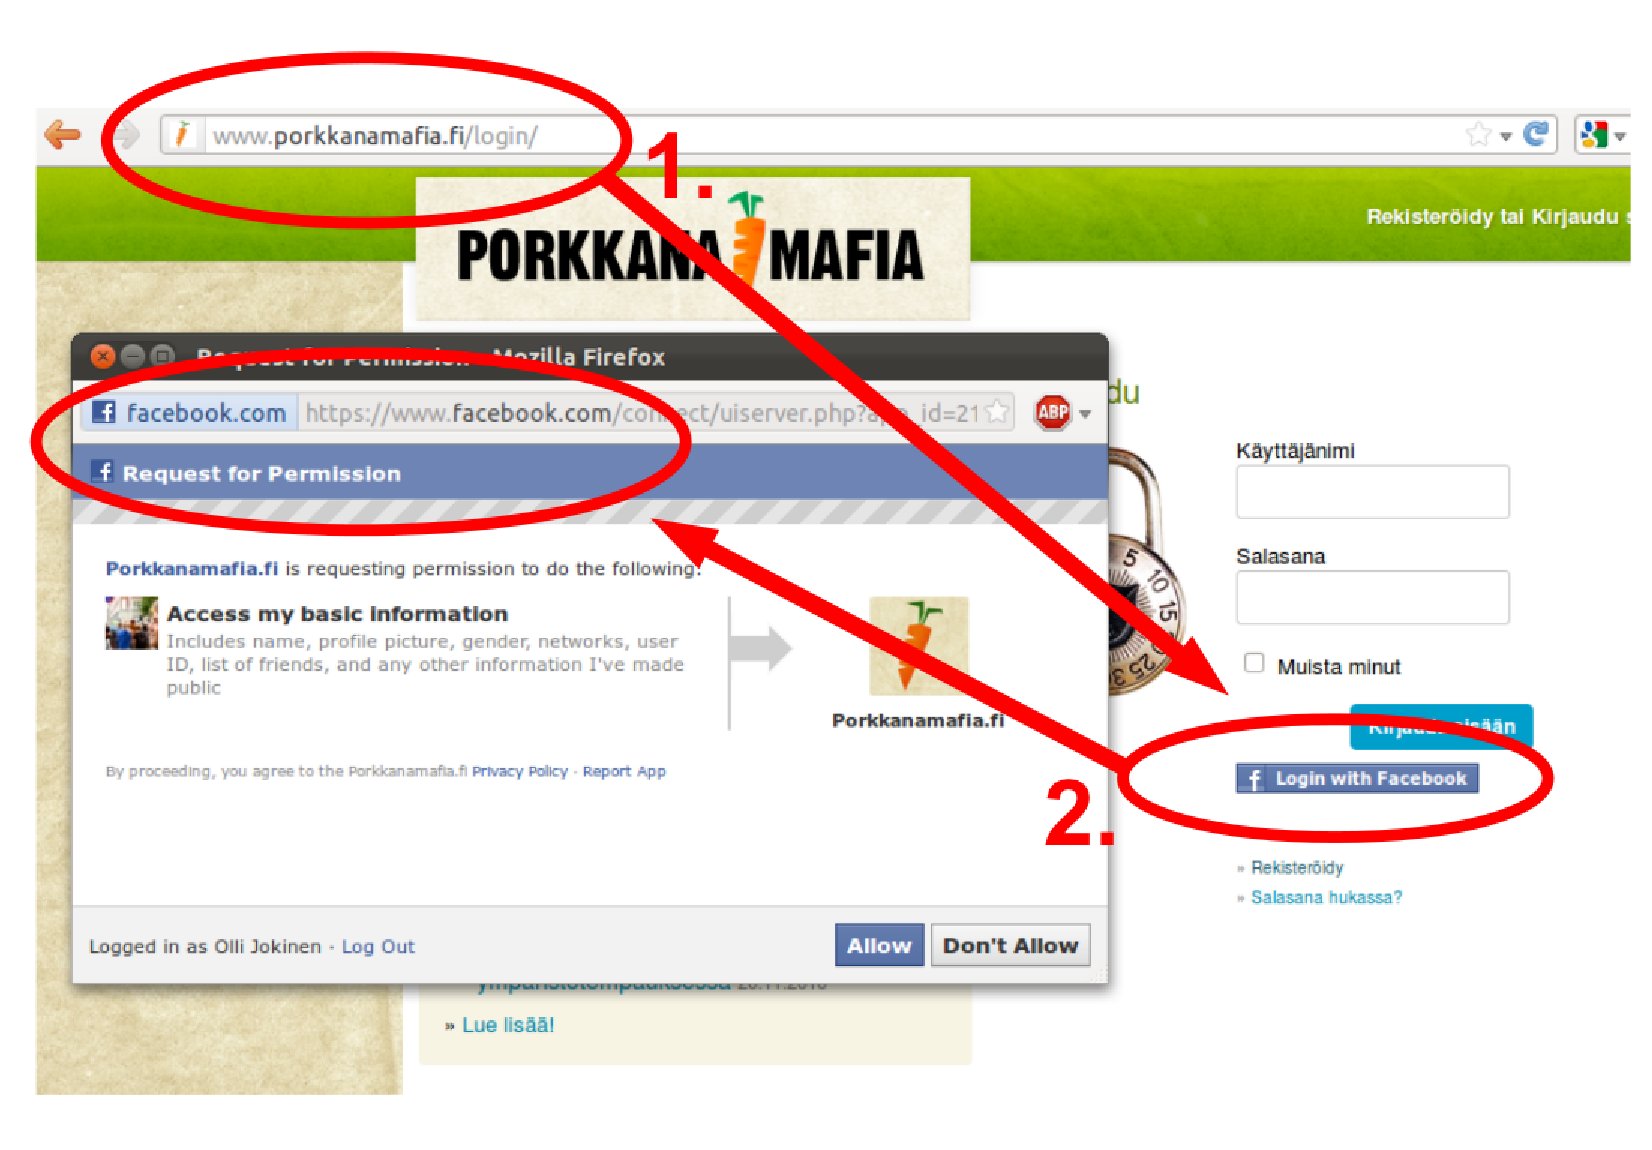
\includegraphics[width=0.7\textwidth]{teknologiat/facebook.eps}
\caption{Käyttäjän kirjautuminen Facebook-tunnuksilla Porkkanamafian web-palveluun.}%
\label{facebook_login}
\end{figure}
\subsection{Keskitetyn tunnistautumisen rajapintaprotokollat}
Tunnistautumiseen liittyvien käsitteiden läpikäynti ennen protokollien yksityiskohtaista esittelyä auttaa tunnistautumiseen liittyvien periaatteiden hahmottamista. Käsitteet ovat yleisluontoisia ja eivätkä kosketa vain tiettyjä protokollaa. Protokollien yhteydessä käytetään käsitteitä asiakasohjelma, tunnistautumispalvelu, suojattu resurssi, valtuutustieto (credentials), valtuutusavain (authorization code) ja pääsyvaltuutus (access token) \cite{nisti}.

Asiakasohjelmalla tarkoitetaan web-palvelun käyttäjän pääteohjelmaa, jolla hän kirjautuu web-palveluun käyttäen keskitettyä tunnistautumispalvelua. Käytännössä asiakasohjelma on web-palvelun tapauksessa käyttäjän WWW-selain, joka pystyy tekemään uudelleenohjauksia sivustolta toiselle. Uudelleenohjaus on HTTP-protokollan perustoiminnallisuutta, joten mikä tahansa HTTP/1.1-standardin WWW-selain käy asiakasohjelmaksi \cite{rfc2616}.

Tunnistautumispalvelu on web-palvelu, johon käyttäjä ohjataan tekemään tunnistautuminen. Onnistuneen tunnistautumisen jälkeen tunnistautumispalvelu ohjaa asi\-a\-kas\-oh\-jel\-man takaisin tunnistautumista pyytäneen palvelun määrittelemään osoitteeseen \cite{nisti}. Avoimen Internetin puolella tunnistautumispalvelu voi olla esimerkiksi Facebook tai LinkedIn.

Tunnistautumisprotokollien yhteydessä suojatulla resurssilla tarkoitetaan resurssia, jonka käyttö vaatii tunnistautumisen ja käyttöoikeuden. Yleisessä tapauksessa suojatulla resurssilla tarkoitetaan yksittäistä resurssia (käyttäjän valokuvaa), johon halutaan asettaa pääsyrajoituksia \cite{nisti}. Tämän tutkielman puitteissa suojatulla resurssilla tarkoitetaan tunnistautumista vaativaa web-palvelua.

Valtuutustieto koostuu yksilöivästä tunnisteesta ja siihen liittyvästä salaisesta avaimesta. Tämän tutkielman puitteissa valtuutustiedolla tarkoitetaan käyttäjän tunnusta ja salasanaa.

Kirjauduttuaan sisään tunnistautumispalvelimelle, käyttäjä saa valtuutusavaimen, jonka hän lähettää eteenpäin suojatun resurssin omistajalle. Valtuutusavain ei pidä sisällään käyttäjän valtuutustietoja, vaan ainoastaan tunnistautumispalvelin osaa lukea sen \cite{nisti}. Saatuaan valtuutusavaimen käyttäjältä voi suojatun resurssin omistaja hakea pääsyvaltuuden käyttäjän tietoihin tunnistautumispalvelusta.

Pääsyvaltuutus on tunnistautumispalvelimelta saatava yksilöivä tunniste, jonka avulla suojatun resurssin omistaja voi pyytää käyttäjän tiedot tunnistautumispalvelulta. Pääsyvaltuutus on voimassa tietyn ajan, jonka jälkeen se täytyy uusia tunnistautumispalvelimella \cite{nisti}. Pääsyvaltuutusta voidaan käyttää myös tunnistautumispalvelusta erillään olevien resurssien valtuuttamiseen. Esimerkiksi web-sovellus voi hakea tunnistautumispalvelulta pääsyvaltuuden, jolla hän hakee valokuvia valokuvien jakopalvelusta \cite{facebook}.
\subsubsection{Rajapintaprotokollien toimintaperiaate}
Tunnistautumisessa on kolme osapuolta: asiakasohjelma, web-palvelu ja tunnistautumispalvelu \cite{nisti}. Osapuolet on esitetty kuvassa \ref{composition}, jossa on mukana myös tunnistautumispalvelun käyttämä käyttäjähallinta. Käyttäjähallinta voi olla myös osa tunnistautumispalvelua tai oma komponenttinsa. Tunnistautumisen kannalta sillä, onko käyttäjähallinta osa tunnistautumispalvelu vai erillinen komponentti, ei ole väliä.

\begin{figure}[ht]
\centering
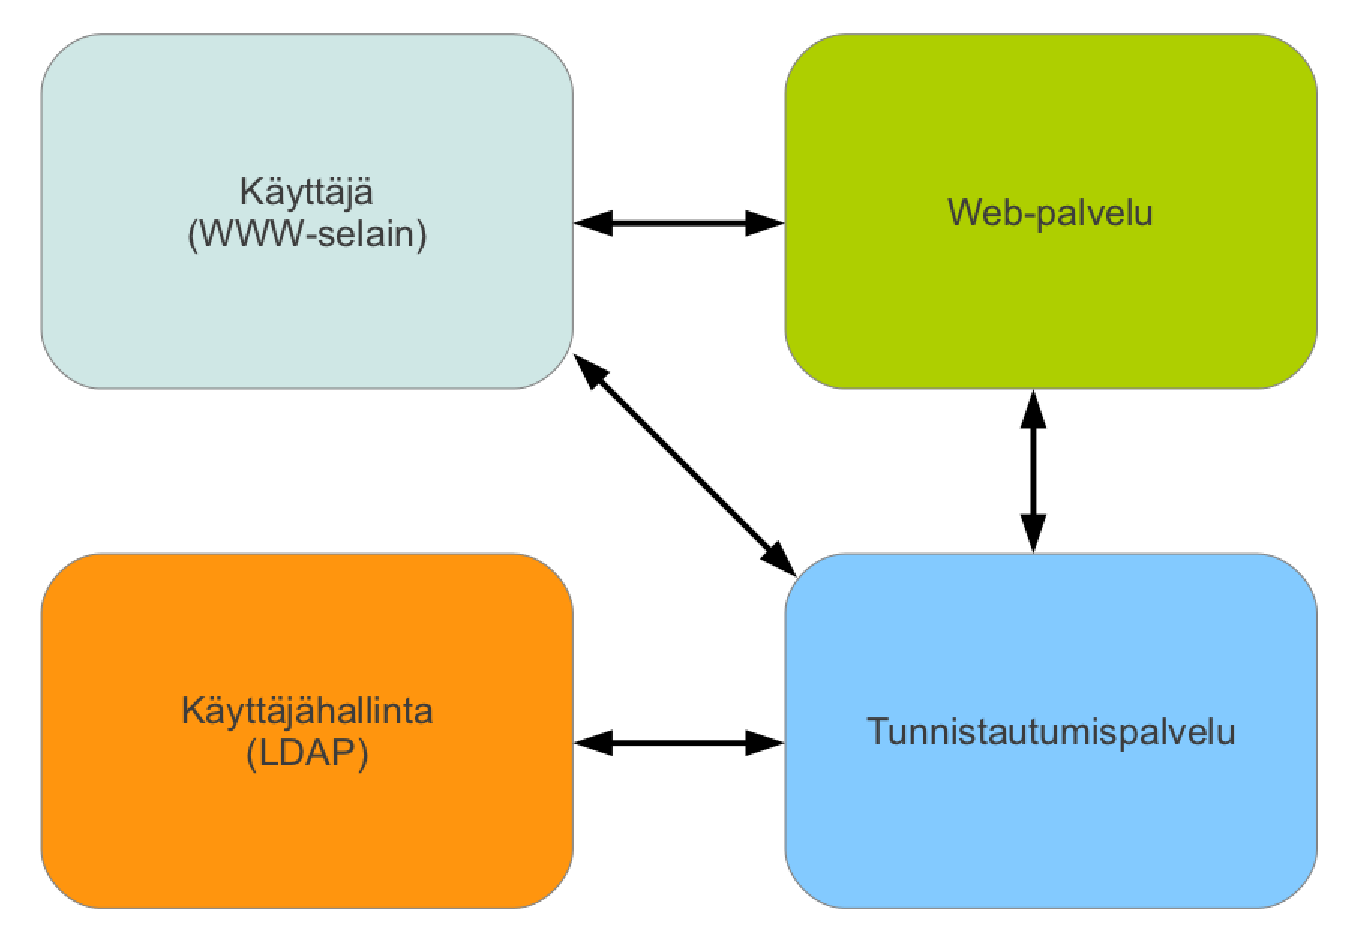
\includegraphics[width=0.7\textwidth]{teknologiat/composition.eps}
\caption{Keskitetyn tunnistautumisen osapuolet.}%
\label{composition}
\end{figure}

Kuvassa \ref{oauth} on tunnistautumisprotokollien sekvenssikaavio, jossa on kuvattu vaiheet käyttäjän kirjautuessa web-palveluun. Ensimmäiseksi käyttäjä menee asiakasohjelmalla web-palveluun, joka pyytää tunnistautumista erillisessä tunnistautumispalvelussa. Käyttäjän asiakasohjelma ohjataan tunnistautumispalvelun sivulle, joka on yhteydessä organisaation käyttäjähallintaan. Jos käyttäjähallinnasta löytyvät käyttäjän syöttämät tunnistetiedot, palautetaan käyttäjälle valtuutusavain, jonka käyttäjä lähettää takaisin web-palvelulle \cite{nisti}. Tämän jälkeen web-palvelu varmistaa tunnistautumispalvelulta valtuutusavaimen oikeellisuuden ja tunnistautumispalvelu palauttaa käyttäjän tiedot web-palvelulle.

Useimmat tunnistautumisen vaiheet tapahtuvat käyttäjältä näkymättömissä selaimen uudelleenohjauksella. Käyttäjälle näkyvät vaiheet ovat 4 ja 5, joissa käyttäjältä pyydetään käyttäjätunnus ja salasana sekä varmistetaan tietojen lähetys web-palveluun. Käyttäjän syötettä vaativat vaiheet on esitetty aiemmassa kuvassa \ref{facebook_login}.

\begin{figure}[ht]
\centering
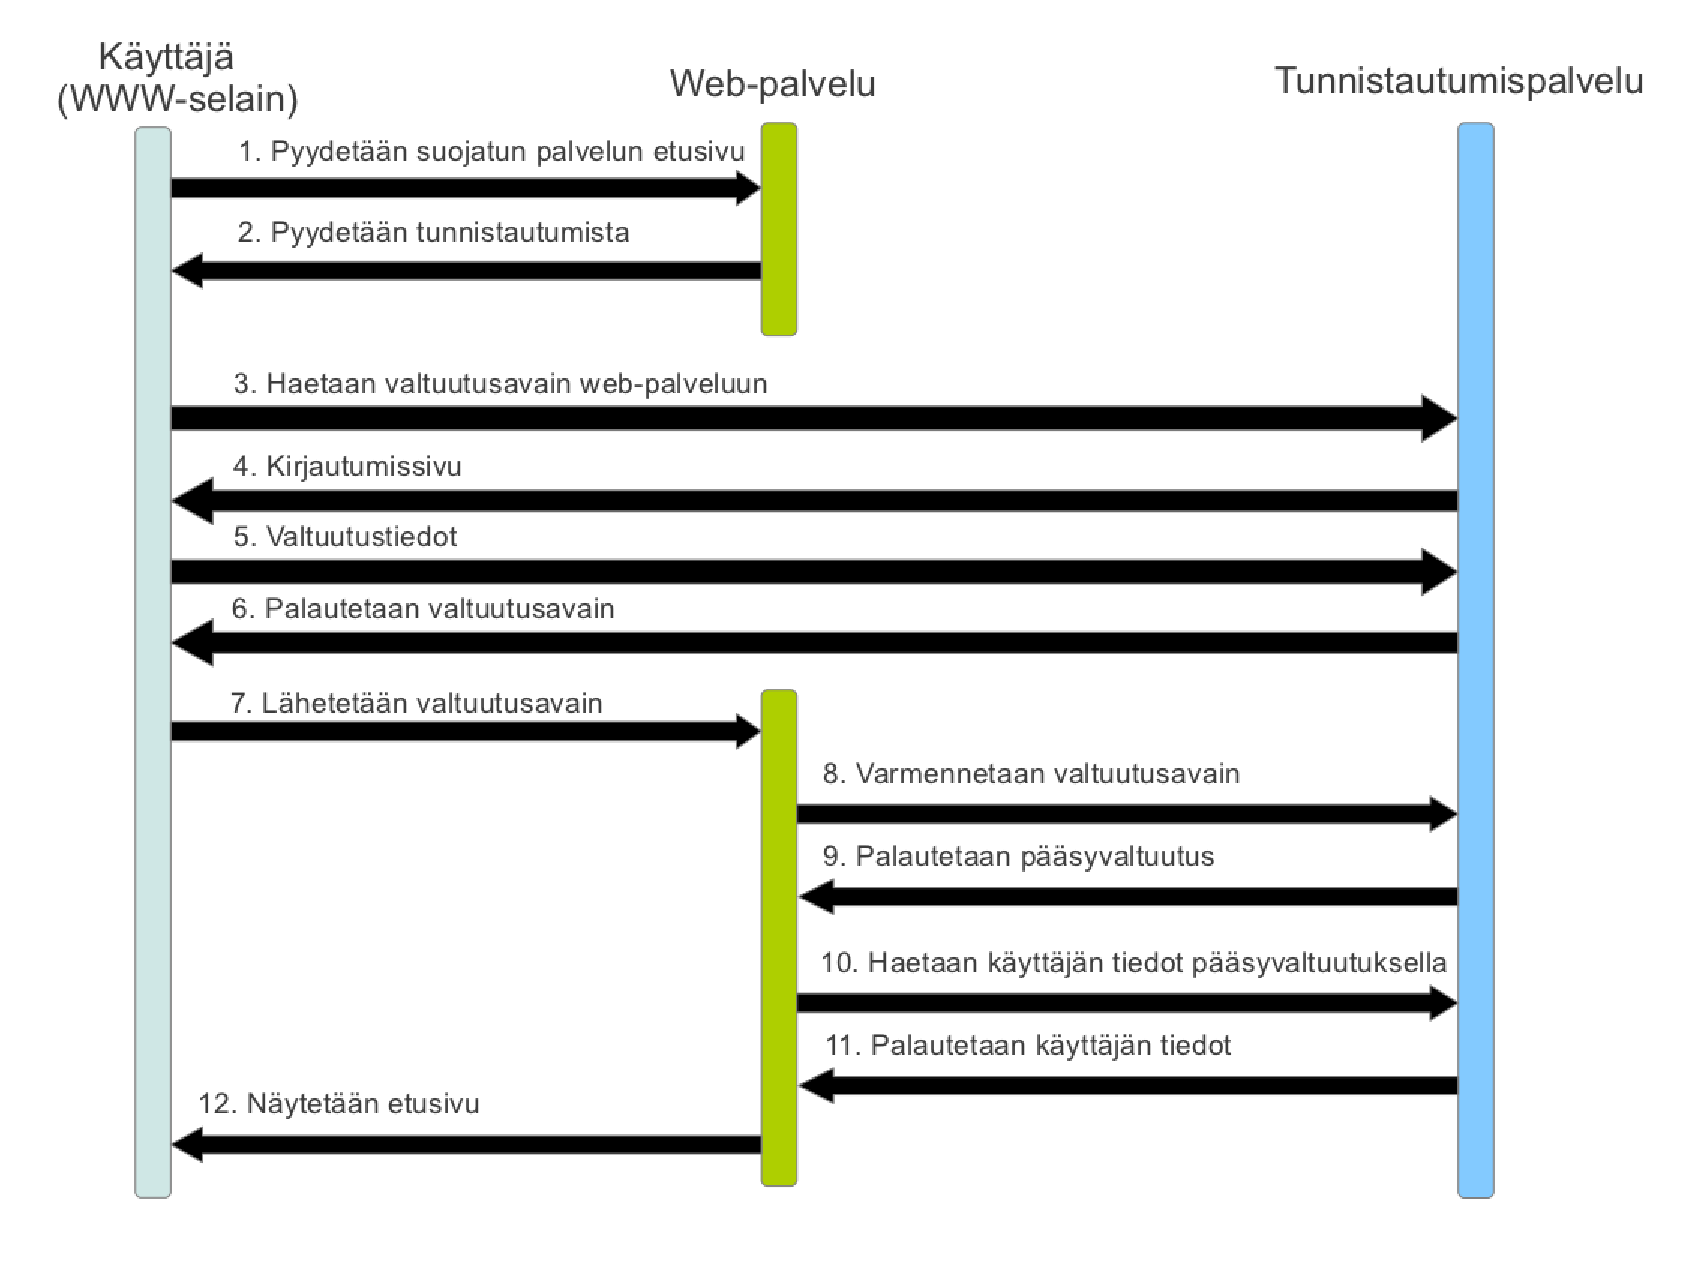
\includegraphics[width=\textwidth]{teknologiat/protokollat/oauth.eps}
\caption{Tunnistautuminen sekvenssikaaviona.}%
\label{oauth}
\end{figure}
\subsubsection{Rajapintaprotokollien standardeja}
Tunnistautumisprotokollia tutkitaan ja kehitetään monen eri tahon toimesta. Web Services -teknologioita standardoinut OASIS (Organization for the Advancement of Structured Information Standards) on kehittänyt XML-pohjaista SAML-kieltä tunnistautumisprotokollaksi \cite{saml_spec}. SAML tarjoaa tunnistautumisprotokollan lisäksi joukon muita web-sovellukseen liittyviä turvallisuusstandardeja \cite{next_saml}.

Myös Microsoft on kehittänyt oman Windows Live ID -standardin, joka tarjoaa tunnistautumisprotokollan \cite{open_identity}. Windows Live ID on osittain suljettu standardi, joka tarjoaa tunnistautumisprotokollien lisäksi täydellisen keskitetyn käyttäjän identiteetin hallinnan \cite{open_identity}. Suljetun lähdekoodin vuoksi Windows Live ID ei ole tämän tutkielman kannalta kiinnostava protokolla.

Avoimen lähdekoodin yhteisössä on syntynyt OpenID, jota mm. Google käyttää tunnistautumisprotokollanaan \cite{open_identity}. OpenID:stä on kehittynyt OAuth-pro\-to\-kol\-la, joka on tarkoitettu nimenomaan pääsynhallintaan, mutta jolla voidaan toteuttaa myös tunnistautuminen \cite{formal_oauth}. OpenID ja OAuth ovat tämän tutkielman kannalta kiinnostavia teknologioita, sillä ne ovat avoimia ja niiden kehitystyö on aktiivista \cite{facebook}. OpenID:n, OAuthin ja SAML:n ominaisuuksia ja soveltuvuutta keskitetyn tunnistautumispalvelun rajapintaprotokollaksi tarkastellaan seuraavissa alaluvuissa.
\subsubsection{SAML}
Security Assertion Markup Language (SAML) on OASIS-komitean määrittelemä XML-pohjainen avoin standardi tunnistautumiseen ja pääsynhallintaan \cite{saml_spec}. Standardin versio 1.0 julkaistiin marraskuussa 2002 ja versio 2.0 maaliskuussa 2005. Version 2.0:n viimeisin korjattu versio 5 julkaistiin helmikuussa 2012.

SAML määrittelee XML-pohjaiset työkalut tunnistautumisen ja pääsynhallinnan toteuttamiseen. Varsinainen toteutus, esimerkiksi se, mitä tietoja siirretään ja millä tavalla, jätetään SAML:ssä toteuttajan päätettäväksi \cite{dynamic_saml}. Varsinaiset SAML-viestit voivat kulkea esimerkiksi synkronisesti SOAP- ja HTTP-protokollalla. SAML soveltuu avoimena ja XML-pohjaisena protokollana käytettäväksi Web Services -standardilla toteutetuissa web-sovelluksissa.

Standardi koostuu useista eri komponenteista, jotka yhdessä muodostavat SAML v2.0 -spesifikaation \cite{saml_spec}. Keskeisempänä ovat vakuutukset (assertion), joihin sovellukset voivat luottaa. Nämä vakuutukset koskevat tunnistautumista, pääsynvalvontaa sekä attribuutteja. SAML:ssa on määritelty myös protokollasidokset (protocol bindings), joiden mukaan vakuutukset siirtyvät järjestelmästä toiseen. Yhdessä nämä muodostavat profiileja, joiden avulla esimerkiksi keskitetty tunnistautuminen voidaan toteuttaa \cite{saml_spec}.

SAML on vakiintunut standardi ja siihen on määritelty erilaisia laajennoksia, joiden ansiosta samalla standardilla voidaan toteuttaa koko identiteentinhallinta \cite{saml_spec}. Tästä syystä se on vakiintunut standardina erityisesti yritysten sisäisissä kertakirjautumisratkaisuissa (Single Sign On) \cite{dynamic_saml}. Kuitenkaan niin kutsutun julkisen Internetin puolella SAML ei ole saavuttanut merkittävää asemaa, vaan yritykset kuten Google ja Facebook ovat toteuttaneet omat tunnistautumisrajapintansa kevyemmillä protokollilla, kuten OpenID:llä ja OAuthilla.
\subsubsection{OpenID}
OpenID standardin ensimmäisen version on kehittänyt toukokuussa 2005 Brad Fitzpatrick [TODO: lähde]. Tuoreimman 2.0 version kehitys aloitettiin 2007 ja sen kehitys on edelleen aktiivista. Se on SAMLia rajoitetumpi protokolla, jonka tavoite on käyttäjätunnuksen käytön mahdollistaminen eri web-palveluissa. Nykyään sen kehityksestä vastaa OpenID Foundation -säätiö, jonka jäsenenä on mm. Google ja Microsoft [TODO: lähde].

OpenID-palveluntarjoaja tarjoaa päätepisteen (endpoint), johon web-palvelut voivat tunnistautua. Tunnistautumiseen voidaan käyttää kahta erilaista virtausta (flow).  Suunnatussa identiteetin (directed identity) virtauksessa käyttäjä valitsee palveluntarjoajan, jonka kautta kirjautuminen suoritetaan [TODO: lähde]. Väitetyn identiteetin (claimed identity) virtauksessa web-palvelu hakee päätepisteen annetun OpenID-tunnisteen perusteella [TODO: lähde]. Virtaukset eroavat toisistaan vain vaiheessa, jossa etsitään päätepiste. Kuvassa \ref{openid_flow} on esitetty OpenID-kirjautumisen vaiheet.

\begin{figure}[ht]
\centering
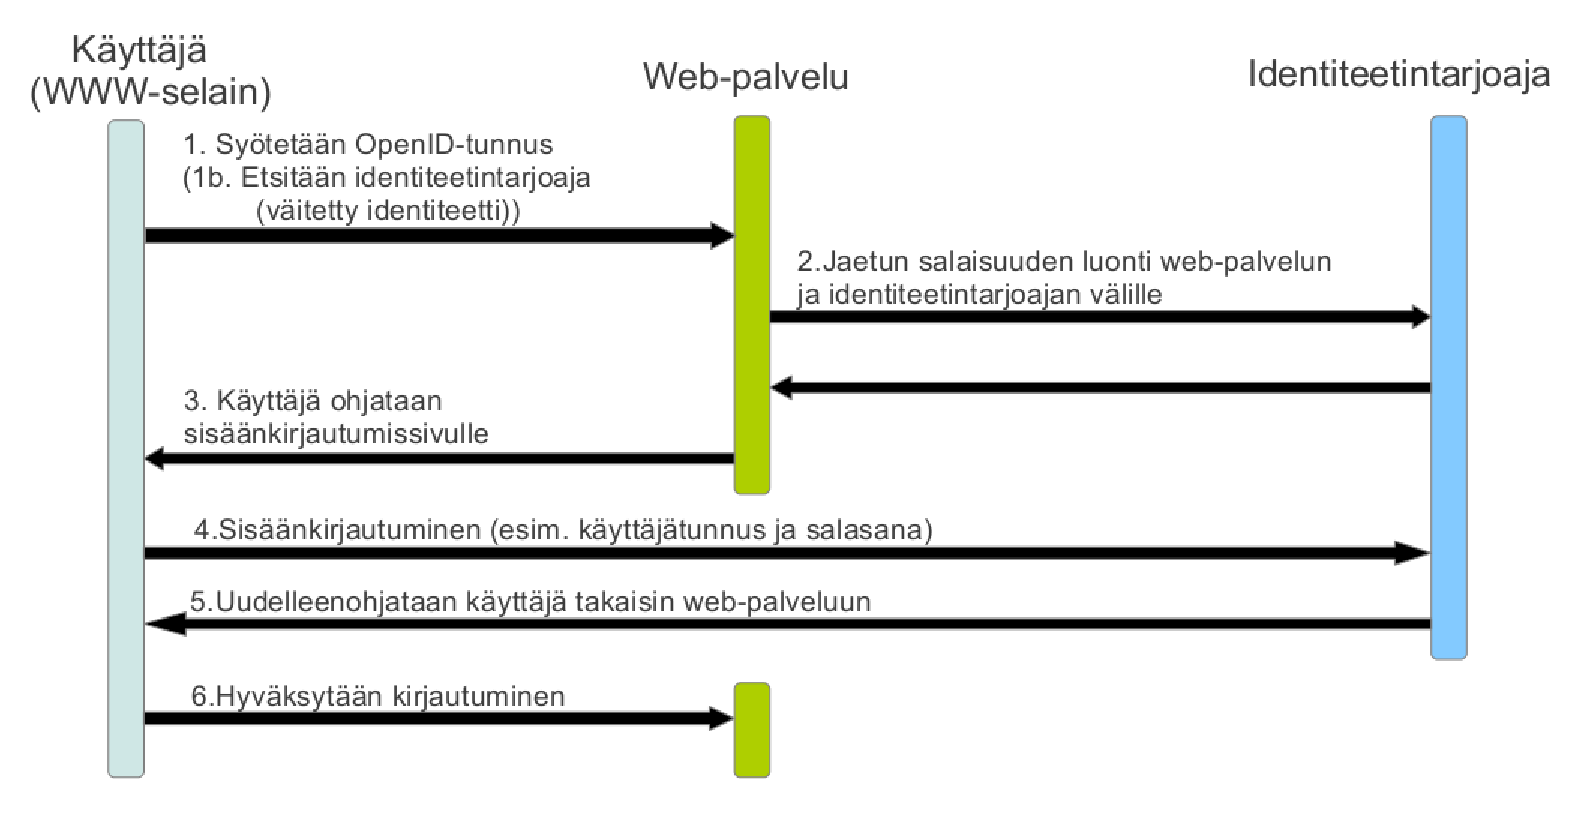
\includegraphics[width=\textwidth]{teknologiat/protokollat/openid.eps}
\caption{OpenID kirjautumisen vaiheet \cite{openid}.}%
\label{openid_flow}
\end{figure}

OpenID:n suhteen odotukset olivat alkujaan suuria, mutta myöhemmin into protokollan ympärillä on laantunut [TODO: lähde]. Esimerkiksi Microsoft vuonna 2008 aloittama OpenID-kokeilu on sittemmin lopetettu ja Microsoft on siirtynyt käyttämään omaa tunnistautumistoteutusta [TODO: lähde]. Yleiset OpenID-kirjautumissivut on korvattu eri palveluntarjoajien kirjautumissivuilla, koska käyttäjätutkimusten mukaan käyttäjät eivät tunne OpenID:tä, mutta tuntevat palveluntarjoajan kuten Googlen tai Yahoon [TODO: lähde]. Näin ollen käyttäjät eivät tiedä kirjautuvansa OpenID:llä palveluun, johon kirjaudutaan Googlen tunnuksilla. Myös alkuperäinen ajatus siitä, että kuka tahansa voi toimia identiteetintarjoajana, on osoittatunut toimimattomaksi, koska web-palveluiden ylläpitäjät haluavat luottaa päätepisteisiin, joiden kautta heidän palveluun voi kirjautua [TODO: lähde].

OpenID:tä lähellä on erillinen OAuth-protokolla, jonka toteutus aloitettiin, kun huomattiin ettei OpenID sovellu kaikkiin tapauksiin. OpenID:stä on kehittynyt myös OpenID Connect, joka paikkaa OpenID:n puutteita [TODO: lähde]. Sen kehitys on kuitenkin vielä niin varhaisessa määrittelyvaiheessa, että sen käyttö tämän tutkielman puitteissa ei ole mielekästä. Sen sijaan OAuth-protokolla on esitelty seuraavassa aliluvussa.
\subsubsection{OAuth}
Tämä kappale tulee luultavasti muuttumaan, yleisiä juttuja johdantoon ja tähän vain Oauth-spesifistä asiaa, miten eroaa kerberoksesta jne. Pituus 2-3 sivua, kuvia yms. Oleellisin näistä protokollista, koska tullaan käyttämään toteutuksessa.

OAuth on avoin tunnistautumisrajapinta hajautetuille web-sovelluksille. Se mahdollistaa käyttäjien resurssien jakamisen palveluiden välillä ilman käyttäjätunnuksen tai salasanan luovuttamista kolmannelle osapuolelle. Se perustuu erilaisten valtuutusavainten (token) välittämiseen palveluiden välillä. OAuth on yleisesti käytössä web-sovelluksissa, joissa halutaan näyttää käyttäjälle kuuluvia resursseja (esimerkiksi valokuvia), jotka sijaitsevat toisessa sovelluksessa [TODO: lähde].

OAuth on määritelty RFC-dokumentissa numero 5849. Sen ensimmäinen versio (1.0) julkaistiin lokakuussa 2007 ja päivitetty versio (1.0a) kesäkuussa 2009 \cite{oauth2_0}. OAuthin versio 2.0 on myös kehitteillä ja se on tarkoitus julkaista marraskuussa 2012 \cite{oauth2_0}.

Alunperin OAuthin kehitystyö alkoi marraskuussa 2006, kun Blaine Cook kehitty Twitter-palveluun OpenID-tukea.

... tarvitaanko tätä?

\begin{figure}[ht]
\centering
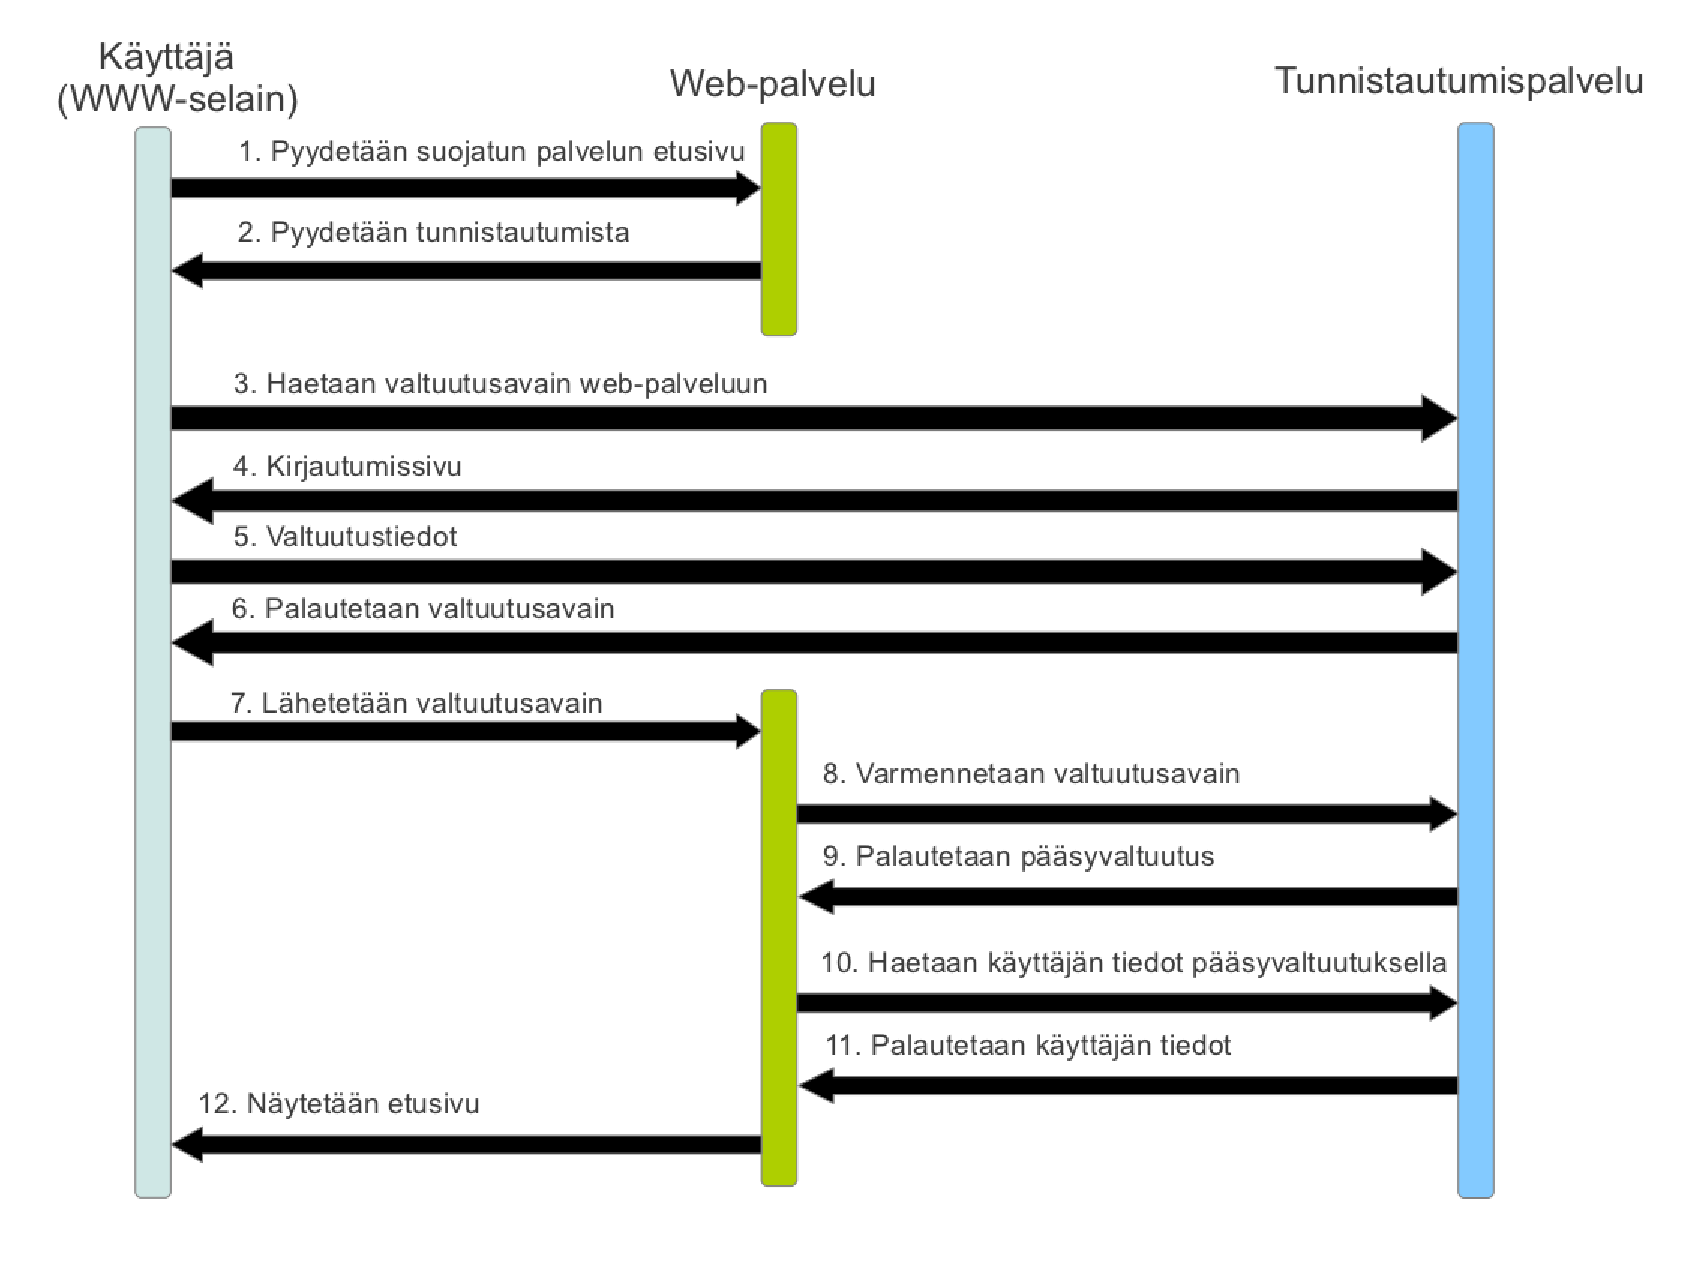
\includegraphics[width=\textwidth]{teknologiat/protokollat/oauth.eps}
\caption{OAuth sekvenssikaavio}%
\label{oauth}
\end{figure}

\subsection{Yhteenveto}
Käytetään OAuthia protossa, koska OpenID:ssä kaikkea tarpeetonta mukana. SAML taas skipataan, koska...? Tätä pitäisi pohtia jossain kohtaa.
